%---------------------------------------------------------------------
% Course 	: Introduction To web sciences
% Professor : Dr.Nelson
% Name   	: Msnoj Chandra Kompalli
% Assignment: 9
%---------------------------------------------------------------------
\documentclass[12pt]{article}
%--------------------------------------------------------------------
% packages required
%--------------------------------------------------------------------
\usepackage{longtable}
\usepackage{graphicx}
\usepackage{listings}
\usepackage{hyperref}
\usepackage{caption}
\usepackage{color}
\usepackage{pdfpages}
\graphicspath{ {images/} }
%--------------------------------------------------------------------
% Start Margins
%--------------------------------------------------------------------
\addtolength{\oddsidemargin}{-.875in}
\addtolength{\evensidemargin}{-.875in}
\addtolength{\textwidth}{1.75in}
\addtolength{\topmargin}{-.885in}
\addtolength{\textheight}{1.95in}
%-------------------------------------------------------------------
% End Margins
%--------------------------------------------------------------------
\definecolor{codegreen}{rgb}{0,0.6,0}
\definecolor{codegray}{rgb}{0.5,0.5,0.5}
\definecolor{codepurple}{rgb}{0.58,0,0.82}
\definecolor{backcolour}{rgb}{0.95,0.95,0.92}
 
\lstdefinestyle{mystyle}{
    backgroundcolor=\color{backcolour},   
    commentstyle=\color{codegreen},
    keywordstyle=\color{magenta},
    numberstyle=\tiny\color{codegray},
    stringstyle=\color{codepurple},
    basicstyle=\footnotesize,
    breakatwhitespace=false,         
    breaklines=true,                 
    captionpos=b,                    
    keepspaces=true,                 
    numbers=left,                    
    numbersep=5pt,                  
    showspaces=false,                
    showstringspaces=false,
    showtabs=false,                  
    tabsize=2
}
 
\lstset{style=mystyle}

\begin{document}

\begin{titlepage}
\title{INTRODUCTION TO WEB SCIENCES:\\*Assignment 9}
\author{Manoj Chandra Kompalli}
\date{21 April 2016}
\maketitle
\end{titlepage}

\tableofcontents
\newpage

\section{Question 1:  }
1.  Choose a blog or a newsfeed (or something similar with an Atom
or RSS feed).  Every student should do a unique feed, so please
"claim" the feed on the class email list (first come, first served).
It should be on a topic or topics of which you are qualified to
provide classification training data.  Find something with at least
100 entries (or items if RSS).

\subsection{Approach}
A blog with more than 100 feeds was really a huge task. Most blogs had around 30 feeds. I had actually tried using a blog about astronomy. I could not categorize the items easily in that blog because most of the items were related.
\begin{itemize}
  \item I have used a newspaper blog’s  sports page.
  \item The Newspaper is Indian Express. As it is an Indian Newspaper, all the sports articles are about the sports followed in India.
  \item Cricket is big in India and most articles are based on it.
 \item Football is a world sport so I found most articles about it.
 \item  As the Rio Olympics are approaching, some data was about it. \item  Tennis is also a big sport and currently many events are taking place all over the worls
 \item Hockey is iIndia's national sport and so some articles could be of that
 \item For sports like WWE, Mototsports I have the category Others
\end{itemize}



 \newpage




\subsection{Input blog data }
\begin{figure}[ht]
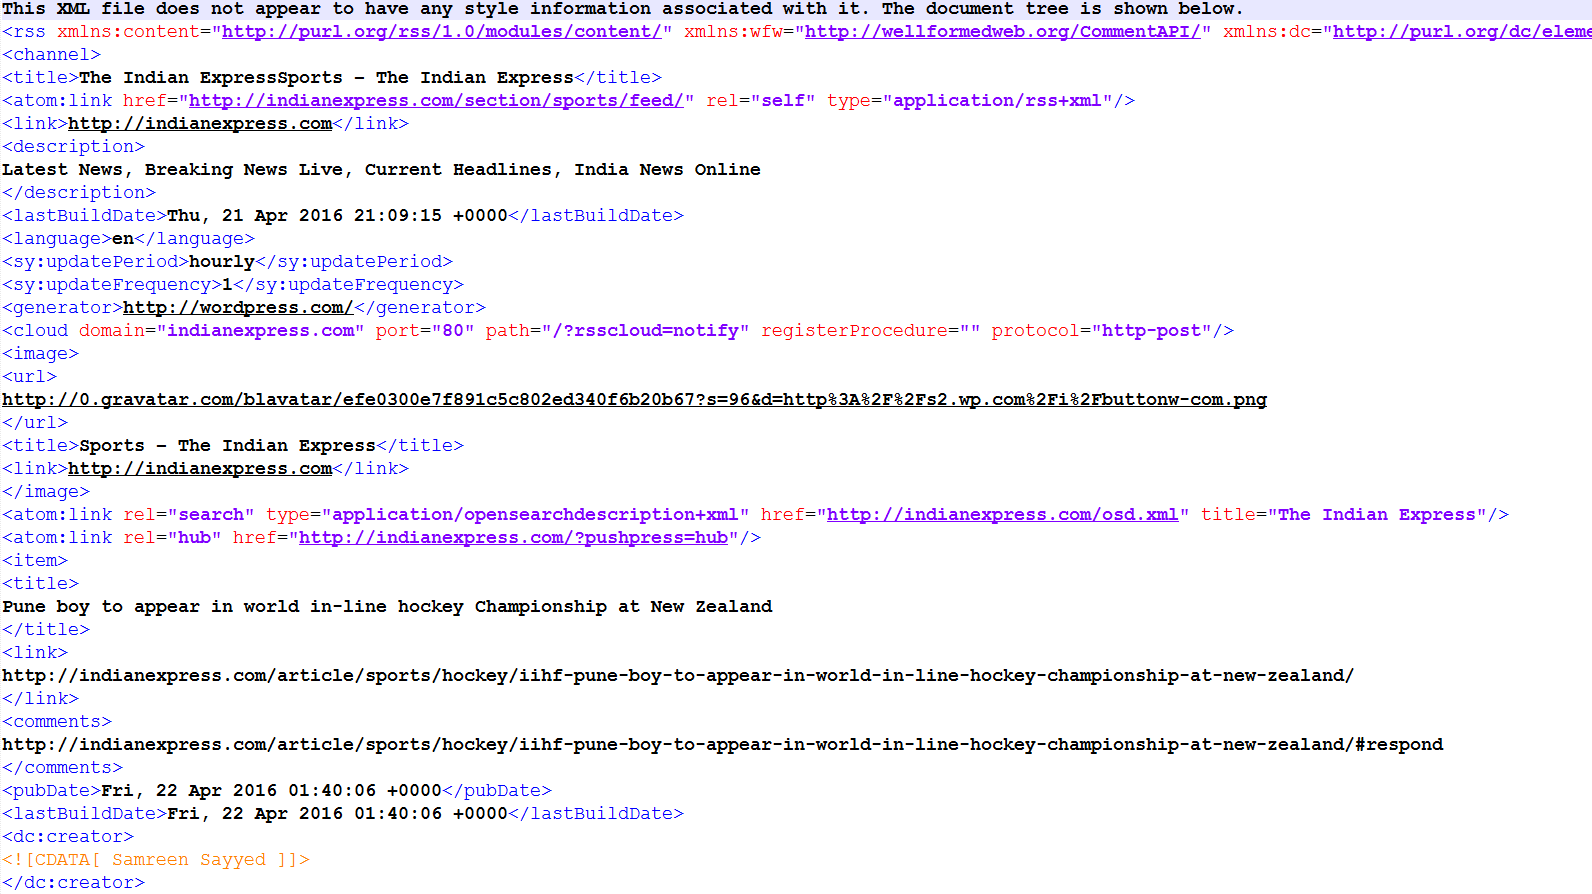
\includegraphics[scale=0.7]{../../q1/input.png}
\centering
\caption{Blog data in xml file containing 100 items}
\label{Removed edges}
\end{figure}


\newpage
\section{Question 2: }
2.  Manually classify the first 50 entries, and then classify (using
the fisher classifier) the remaining 50 entries. 

Create a table with the title, predicted category, actual category,
and cprob() and fisherprob() for the actual category.

\subsection{Approach}
I have started off by training the first 50 words. I have used methods like classify, fisherprob, cprob from docclass.py and feedfilter.py .
Initially most predictions were incorrect but as the training progressed there were good number of hits mostly in categories like cricket and football.

\begin{itemize}
\item I have extracted fisherprob and cprob using the functions  from docclass.
\item Listings show Fisher method used which predicts category based on the entry.
\item Based on the first 50 tarained entries, next 50 categories were predicted.
\item I am showing title,actual,predicted for the first 50 feeds.
\item I am displaying Title,actual,predicted,,cprob,fprob for the last 50 blog items
\end{itemize}
\subsection{Tables}
\subsubsection{Manual Classification}
\begin{longtable}{ |p{2.0cm} | p{10.0cm} | p{2.0cm} |p{2.0cm}| }\hline
\textbf{No.} & \textbf{Title} & \textbf{Predicted} & \textbf{Actual} \\\hline
1 &  Pune boy to appear in world in-line hockey Championship at New Zealand  & None & hockey \\\hline										
2 &  Leicester City and Spurs dominate Players of the Year selection  & hockey & football \\\hline										
3 &  Chris Gayle readies to unwind after birth of daughter ‘Blush’ & hockey & cricket \\\hline										
4 &  Virat Kohli, Ishant Sharma, Ajinkya Rahane, Irfan Pathan indulge in charitable work & hockey & cricket \\\hline										
5 &  Leicester City’s Jamie Vardy accepts FA charge, awaits decision on ban & football & football \\\hline										
6 &  Rafael Nadal beats Albert Montanes to reach Barcelona Open quarterfinals & hockey & tennis \\\hline										
7 &  Louis Oosthuizen joins Vijay Singh, Adam Scott to give Rio Olympics golf a miss & hockey & olympics \\\hline										
8 &  IPL 2016: Sunrisers Hyderabad tame the Lions in their own backyard & football & cricket \\\hline										
9 &  It took ‘guts’ to pick Marcus Rashford, says Manchester United boss Louis Van Gaal & football & football \\\hline										
3 &  Chris Gayle readies to unwind after birth of daughter ‘Blush’ & hockey & cricket \\\hline										
4 &  Virat Kohli, Ishant Sharma, Ajinkya Rahane, Irfan Pathan indulge in charitable work & hockey & cricket \\\hline										
5 &  Leicester City’s Jamie Vardy accepts FA charge, awaits decision on ban & football & football \\\hline										
6 &  Rafael Nadal beats Albert Montanes to reach Barcelona Open quarterfinals & hockey & tennis \\\hline										
7 &  Louis Oosthuizen joins Vijay Singh, Adam Scott to give Rio Olympics golf a miss & hockey & olympics \\\hline										
8 &  IPL 2016: Sunrisers Hyderabad tame the Lions in their own backyard & football & cricket \\\hline										
9 &  It took ‘guts’ to pick Marcus Rashford, says Manchester United boss Louis Van Gaal & football & football \\\hline										
17 &  IPL 2016: RCB replace injured Samuel Badree with uncapped South African Tabraiz Shamsi & cricket & cricket \\\hline										
18 &  Gagan Narang, Chain Singh to vie for final spot in Men’s 50m rifle prone & cricket & others \\\hline										
19 &  Cristiano Ronaldo downplays injury, says ‘all good’ & cricket & football \\\hline										
20 &  Jurgen Klopp formula starting to work magic for Liverpool, says James Milner & cricket & football \\\hline										
21 &  ‘Uncle Virat’ Kohli congratulates Chris Gayle on birth of daughter ‘Blush’ & cricket & cricket \\\hline										
22 &  Rio Games count down starts with Olympia torch lighting & cricket & olympics \\\hline										
23 &  I’ve slept with more than 500 women while on tours for West Indies, former seamer Tino Best reveals in upcoming book & hockey & cricket \\\hline										
24 &  We, humans, failed you: Virat Kohli tweets on Shaktiman’s death & cricket & cricket \\\hline										
25 &  I just want to win, says England’s Ben Stokes & cricket & cricket \\\hline										
26 &  Leicester City fairytale sprinkles magic dust on rival fans & football & football \\\hline										
27 &  Jamie Vardy was very unlucky: Roy Hodgson & football & football \\\hline										
28 &  Chyna, former WWE women’s champ, passes away & cricket & others \\\hline										
29 &  Liverpool thrash 10-man Everton 4-0 in Merseyside derby & football & football \\\hline										
30 &  Neymar to play for Brazil at Rio Games 2016, not Copa America & cricket & football \\\hline										
31 &  IPL 2016: KXIP opt for Dharamsala as second ‘home venue’, leave BCCI, HPCA confused & cricket & cricket \\\hline										
32 &  Will look to continue creating history: Dipa Karmakar & cricket & others \\\hline										
33 &  IPL 2016: Krunal Pandya knows his bowling well, says Rohit Sharma & cricket & cricket \\\hline										
34 &  Chris Gayle becomes father to girl ‘Blush’ & cricket & cricket \\\hline										
35 &  Cristiano Ronaldo needs more rest after injury scare, says Zinedine Zidane & football & football \\\hline										
36 &  Matteo Darmian shines as Manchester United beat Crystal Palace 2-0 & football & football \\\hline										
37 &  ICC to discuss structure, scheduling of bilateral series & cricket & cricket \\\hline										
38 &  Madras High Court dismisses PIL against BCCI & cricket & cricket \\\hline										
39 &  Inzamam-ul-Haq took up Pakistan chief selector job on condition of time to prepare squad for World Cup 2019 & cricket & cricket \\\hline										
40 &  Barcelona snap losing streak to thump Deportivo 8-0; Atletico, Real Madrid win to keep league race alive & cricket & football \\\hline										
41 &  IPL 2016: Water woes brew in Jaipur & cricket & cricket \\\hline										
42 &  Chip off old block: Rahul Dravid’s son Samit scores 125 for school team & cricket & cricket \\\hline										
43 &  FIFA U-17 World Cup tournament director buoyed by Narendra Modi’s encouragement & cricket & football \\\hline										
44 &  Jack Wilshere will be available after West Brom, says Arsene Wenger & cricket & football \\\hline										
45 &  Bayern Munich keeper Manuel Neuer signs contract extension to 2021 & cricket & football \\\hline										
46 &  Jose Mourinho, Claudio Ranieri to manage at Old Trafford for charity & football & football \\\hline										
47 &  Usain Bolt’s main goal: to defend the titles, do a threepeat at Rio Olympics 2016 & cricket & olympics \\\hline										
48 &  I want to go and get more goals for Tottenham Hotspur, says Harry Kane & football & football \\\hline										
49 &  Bombay High Court allows BCCI to hold May 1 IPL 2016 MI vs RPS match in Pune & cricket & cricket \\\hline										
50 &  Athletics report: Tourist hurdler, tired athlete and a bumbling walker & cricket & others \\\hline										

 \caption{Entries classified manually}
\end{longtable}
\subsubsection{Last 50 items using fisher classifier }
\begin{longtable}{|p{2.0cm} | p{6.0cm} | p{2.0cm} |p{2.0cm}| p{2.0cm}|p{2.0cm}|}\hline
\textbf{No.} & \textbf{Title} & \textbf{Predicted} & \textbf{Actual} &  \textbf{CProb}  & \textbf{FisherProb}\\\hline
51 & Have to improve my landings, says Dipa Karmakar & cricket & Olympics & 0 & 0.083 \\\hline													
52 & Sports federations concerned about venues for Rio Games 2016 & cricket & Olympics & 0 & 0.25 \\\hline													
53 & KKR put KXIP back in their place – bottom & cricket & cricket & 0 & 0.5 \\\hline													
54 & We have to win, we need to win, says Louis Van Gaal & football & football & 0 & 0.833 \\\hline													
55 & PSG silent over Jose Mourinho reports & football & football & 0 & 0.5 \\\hline													
56 & PM Modi lauds Dipa Karmakar for her determination & football & football & 0 & 0.5 \\\hline													
57 & Pablo Zabaleta casts doubt over Manchester City future & football & football & 0 & 0.5 \\\hline													
58 & From what I’ve heard… Antonio Conte’s disciplined, says Cesc Fabregas & football & football & 0 & 0.5 \\\hline													
59 & Former German FA boss cleared over Qatar ‘cancer’ comment & football & football & 0 & 1 \\\hline													
60 & Formula 1 should stop tinkering with rules: Mercedes boss Toto Wolff & cricket & others & 0 & 0.5 \\\hline													
61 & Vincent Kompany is working 100 percent with normality, says Manuel Pellegrini & football & football & 0 & 0.75 \\\hline													
62 & The performance Tottenham Hotspur showed was perfect, says Mauricio Pochettino & football & football & 0 & 0.75 \\\hline													
63 & SRH vs MI, IPL 2016: David Warner played a great innings, says Tim Southee & cricket & cricket & 0 & 0.955 \\\hline													
64 & Next objective is a medal in Rio Olympics 2016, says Dipa Karmakar & others & olympics & 0 & 0.083 \\\hline													
65 & IPL 2016, SRH vs MI: Barinder Sran fined for inappropriate conduct & cricket & cricket & 0 & 1 \\\hline													
66 & Ex-CBI chief moves High Court over BCCI-ICC revenue model & cricket & cricket & 0 & 0.75 \\\hline													
67 & Suresh Raina, wife Priyanka expecting first child & cricket & cricket & 0 & 0.75 \\\hline													
68 & PCB disappointed after West Indies refuse to tour Pakistan in 2016 & cricket & cricket & 0 & 0.75 \\\hline													
69 & South Africa players against day-night Tests, ‘feel disadvantaged’ & cricket & cricket & 0 & 0.5 \\\hline													
70 & Spurs hit Stoke City for a four, cut Leicester City’s lead & football & football & 0 & 0.875 \\\hline													
71 & Novak Djokovic, Serena Williams wins Laureus World Sportsman and Sportswoman of the Year awards & football & tennis & 0 & 0.5 \\\hline													
72 & Formula One allows Pirelli more track days to test tyres for 2017 & cricket & others & 0 & 0.25 \\\hline													
73 & After win in Monte Carlo, Rafael Nadal turns sights to Barcelona & cricket & tennis & 0 & 0.5 \\\hline													
74 & At Rio Olympics, India plans to promote ‘Make in India’ initiative & olympics & olympics & 0 & 0.87 \\\hline													
75 & One-state, one-vote in BCCI will lead to internal politics, BCA tells Supreme Court & cricket & cricket & 0 & 0.9 \\\hline													
76 & Dipa Karmakar vaults into history books after qualifying for Rio Olympic Games 2016 & others & Olympics & 0 & 0.25 \\\hline													
77 & IPL 2016, SRH vs MI: In David vs Goliath, Warner the difference & cricket & cricket & 0 & 0.75 \\\hline													
78 & Charged with ‘improper conduct’, Jamie Vardy could face extended ban & football & footbal & 0 & 0.5 \\\hline													
79 & Newcastle United hoping Manchester City will be distracted by Champions League semi-final & football & football & 0 & 0.5 \\\hline													
80 & Barcelona’s slump baffles Carles Puyol, Luis Figo, Raul & football & football & 0 & 0.5 \\\hline													
81 & Azlan Shah Cup: A few takeaways for India men’s hockey team & cricket & hockey & 0 & 0.25 \\\hline													
82 & IPL 2016, KXIP vs RPS: All is well that Glenn Maxwell ends & cricket & cricket & 0 & 0.5 \\\hline													
83 & IPL 2016: Who said what about DD’s win over RCB & cricket & cricket & 0 & 0.833 \\\hline													
84 & Bengaluru FC retain I-League title with one game to play & football & football & 0 & 1 \\\hline													
85 & Rafael Nadal is ‘King of Clay’ once again with Monte Carlo title & football & tennis & 0 & 0.25 \\\hline													
86 & Leaving Afghanistan’s coach job costs Inzamam-ul-Haq rupees 4 lakhs & cricket & cricket & 0 & 0.75 \\\hline													
87 & Leicester City, minus Jamie Vardy, salvage 2-2 draw with West Ham United & football & football & 0 & 0.666 \\\hline													
88 & Jurgen Klopp makes 10 changes as Liverpool beat Bournemouth & football & football & 0 & 0.833 \\\hline													
89 & IPL 2016, RCB vs DD: DD beat RCB by 7 wickets & cricket & cricket & 0 & 0.5 \\\hline													
90 & Rajkot police orders inquiry into celebratory firing at Ravindra Jadeja’s wedding & cricket & cricket & 0 & 0.5 \\\hline													
91 & Roy Hodgson plays down Andy Carroll’s Euro 2016 chances & football & football & 0 & 0.5 \\\hline													
92 & Sebastian Vettel hits out at ‘torpedo’ Daniil Kvyat & others & others & 0 & 0.5 \\\hline													
93 & Engine problems force Lewis Hamilton to back of China grid & football & other & 0 & 0.5 \\\hline													
94 & Positive start by Indian shooters in Rio World Cup & others & others & 0 & 0.5 \\\hline													
95 & Harbhajan Singh can take his villa whenever he wants, says Amrapali CMD & football & cricket & 0 & 0.125 \\\hline													
96 & IPL 2016: KKR beat SRH by eight wicket, Gambhir smashes unbeaten 90 & cricket & cricket & 0 & 0.5 \\\hline													
97 & Mitchell Starc ties the knot with girlfriend Alyssa Healy & cricket & cricket & 0 & 0.5 \\\hline													
98 & IPL 2016 preview: Struggling MI face RCB challenge at Wankhede Stadium & cricket & cricket & 1 & 0.955 \\\hline													
99 & IPL 2016, KXIP vs KKR: KXIP seek home comfort against KKR & cricket & cricket & 1 & 0.833 \\\hline													
100 & IPL 2016, RCB vs DD: Quintal de Kock gives Delhi Daredevils heavyweight scalp & cricket & cricket & 1 & 0.5 \\\hline													
 \caption{Entries classified using Fisher Classifier}
\end{longtable}



\subsection{Code Listing}
\subsubsection{feedfilter.py}
\lstinputlisting[breaklines=True,language=Python]{../../q2/feedfilter.py}
\newpage

\subsubsection{prog.py}
\lstinputlisting[breaklines=True,language=Python]{../../q2/prog.py}
\subsubsection{docclass.py}
\lstinputlisting[breaklines=True,language=Python]{../../q2/docclass.py}








\section{Question 3: }
3.  Assess the performance of your classifier in each of your
categories by computing precision, recall, and F-measure.  
\subsection{Approach}
Precision ,Recall and F measure are based on TP(True positive), True Negative(TN), False Positive(FP), False Negative(FN)


\begin{itemize}
\item Precision  is the fraction of retrieved instances that are relevant
\item Precision=TP/(TP+FP)
\item Recall  is the fraction of relevant instances that are retrieved
\item Recall=TP/(TP+FN)
\item F-Measure  is a measure of a test's accuracy. It considers both the precision  and the recall 
\item F1=2TP/(2TP+FP+FN)

\end{itemize}


\subsection{Tables}


\begin{center}
\begin{table}
\begin{tabular}{ |p{3.0cm}|p{3.0cm}| p{3.0cm} | p{3.0cm} |p{3.0cm}| }\hline
\textbf{Category} & \textbf{TP} & \textbf{TN} & \textbf{FP} & \textbf{FN} \\\hline
cricket & 19 & 6 & 1 & 24 \\\hline			
olympics & 1 & 0 & 4 & 45 \\\hline			
football & 16 & 4 & 0 & 30	\\\hline		
tennis  & 0 & 0 & 3 & 47 \\\hline			
hockey  & 0 & 0 & 1 & 49 \\\hline			
others & 1 & 1 & 3 & 45	\\\hline		




\end{tabular}
\caption{TP TN FP FN values of different categories}
\end{table}
\end{center}

\newpage

\begin{center}
\begin{table}
\small
\begin{tabular}{ | p{3.0cm} | p{2.0cm} |p{2.0cm} | p{2.0cm} | }\hline
\textbf{Category} & \textbf{Precision} & \textbf{Recall} & \textbf{F1} \\\hline
cricket & 0.95  &  0.44  & 0.6031 \\\hline			
olympics & 0.2  &  0.02173  & 0.03921 \\\hline			
football & 1  &  0.3478  & 0.5161 \\\hline			
tennis  & 0  &  0  & 0	\\\hline		
hockey  & 0  &  0  & 0	\\\hline		
others & 0.25  &  0.02173  & 0.04 \\\hline			

\end{tabular}
\caption{Precision Recall and F1 values for each category}
\end{table}
\end{center}


\newpage






\addcontentsline{tableofcontents}{section}{References}





\bibliographystyle{plain}
\bibliography{references}
\cite{*}
\end{document}